\section{Interval Scheduling}
\label{sec:interval}
Scheduling problems arise in many areas, such as scheduling classes, tasks, or jobs. Interval scheduling is a type of scheduling problem where we want to maximize the number of tasks we can complete.\\

\begin{Def}[Schedule]
    
    A \textbf{schedule} is a set of tasks which we call \textbf{jobs}. Each job has a start time $s_i$ and an end time $f_i$.
    Two jobs are \textbf{compatible} if they do not overlap.
\end{Def}
\begin{figure}[h]
    \begin{center}
      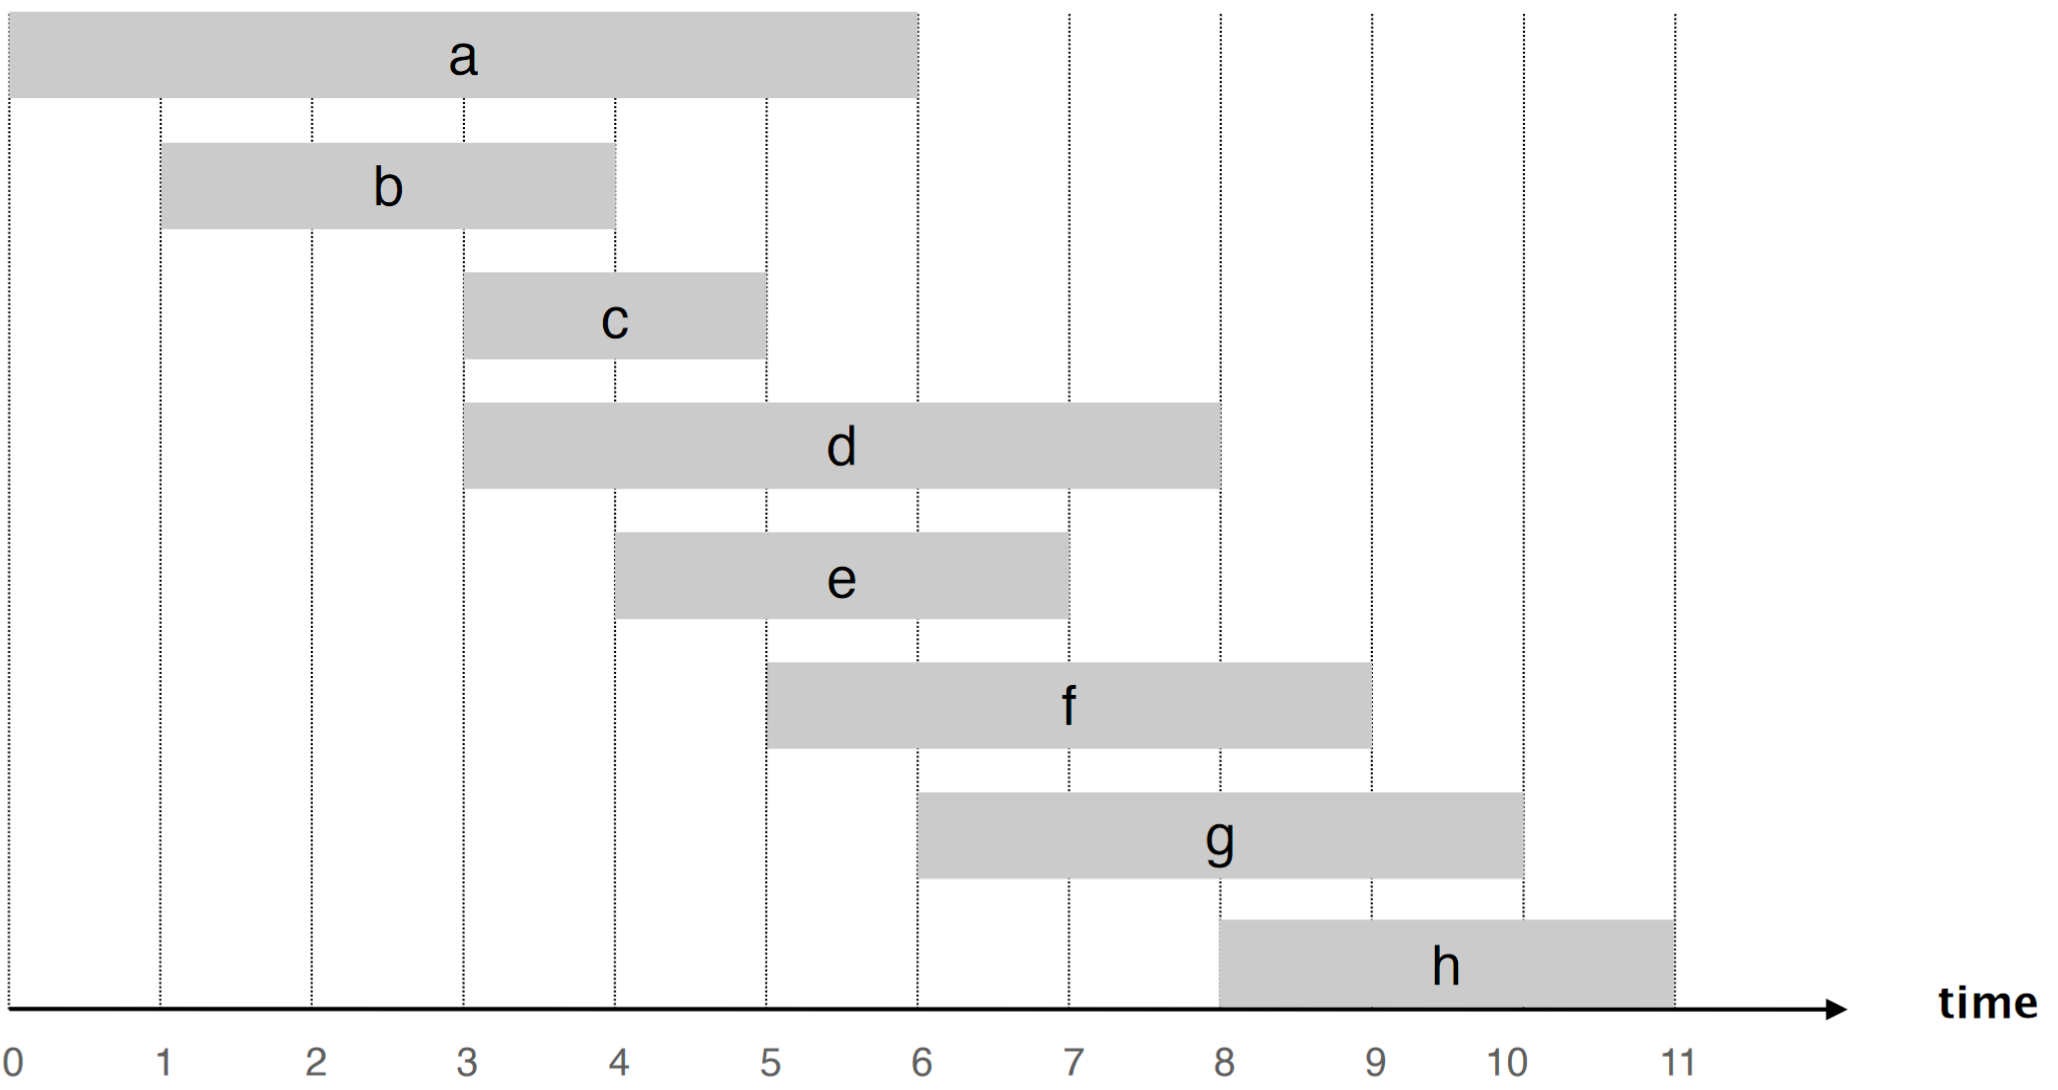
\includegraphics[height=3in]{./Sections/sched/interval/interval.png}
    \end{center}
     \caption{Given jobs $a$ through $h$ we find the largest subset of mutually compatible jobs $\{b,e,h\}$.}\label{fig:interval}
\end{figure}

\newpage

\begin{Def}[Greedy Algorithm]
    
    A \textbf{greedy algorithm} is an algorithm that makes the best choice at each step. I.e.,
    it cares not about the future or big picture, only the immediate benefit, for fast computations.
\end{Def}

\begin{Note}
    \textbf{Note:} This definition becomes \textit{loose}, as we encounter problems with backtracking or multiple states. As in each state
    it makes the best choice with the information available.
\end{Note}

\textbf{Possible Approaches:} Let $s_j$ and $f_j$ be the start and finish times of job $j$.
\begin{itemize}
    \item \textbf{[Earliest Start Time]:} Consider jobs in ascending order of $s_j$.
    \item \textbf{[Earliest Finish Time]:} Consider jobs in ascending order of $f_j$.
    \item \textbf{[Shortest Interval]:} Consider jobs in ascending order of $f_j - s_j$.
    \item \textbf{[Fewest Conflicts]:} For each $j$, count the number of conflicting jobs $c_j$. Schedule in ascending order of $c_j$.
\end{itemize}

\noindent
We choose the \textbf{Earliest Finish Time} approach:
\begin{Proof}[Greedy Algorithm Earliest Finish Time Correctness]
    Let $i_1, i_2, \dots, i_k$ denote the set of jobs selected by the greedy algorithm.
    
    Let $j_1, j_2, \dots, j_m$ denote the set of jobs in an optimal solution, with
    \[
    i_1 = j_1, i_2 = j_2, \dots, i_r = j_r \text{ for the largest possible value of } r.
    \]
    \noindent
    We can swap $j_{r+1}$ for $i_{r+1}$ in the optimal schedule, and it will still remain compatible. We repeat swaps until $r = k$.
    It’s not possible that $m > k$ because $j_{k+1}$ is compatible with $i_k$.
    \end{Proof}
   \begin{figure}[h]
    \begin{center}
      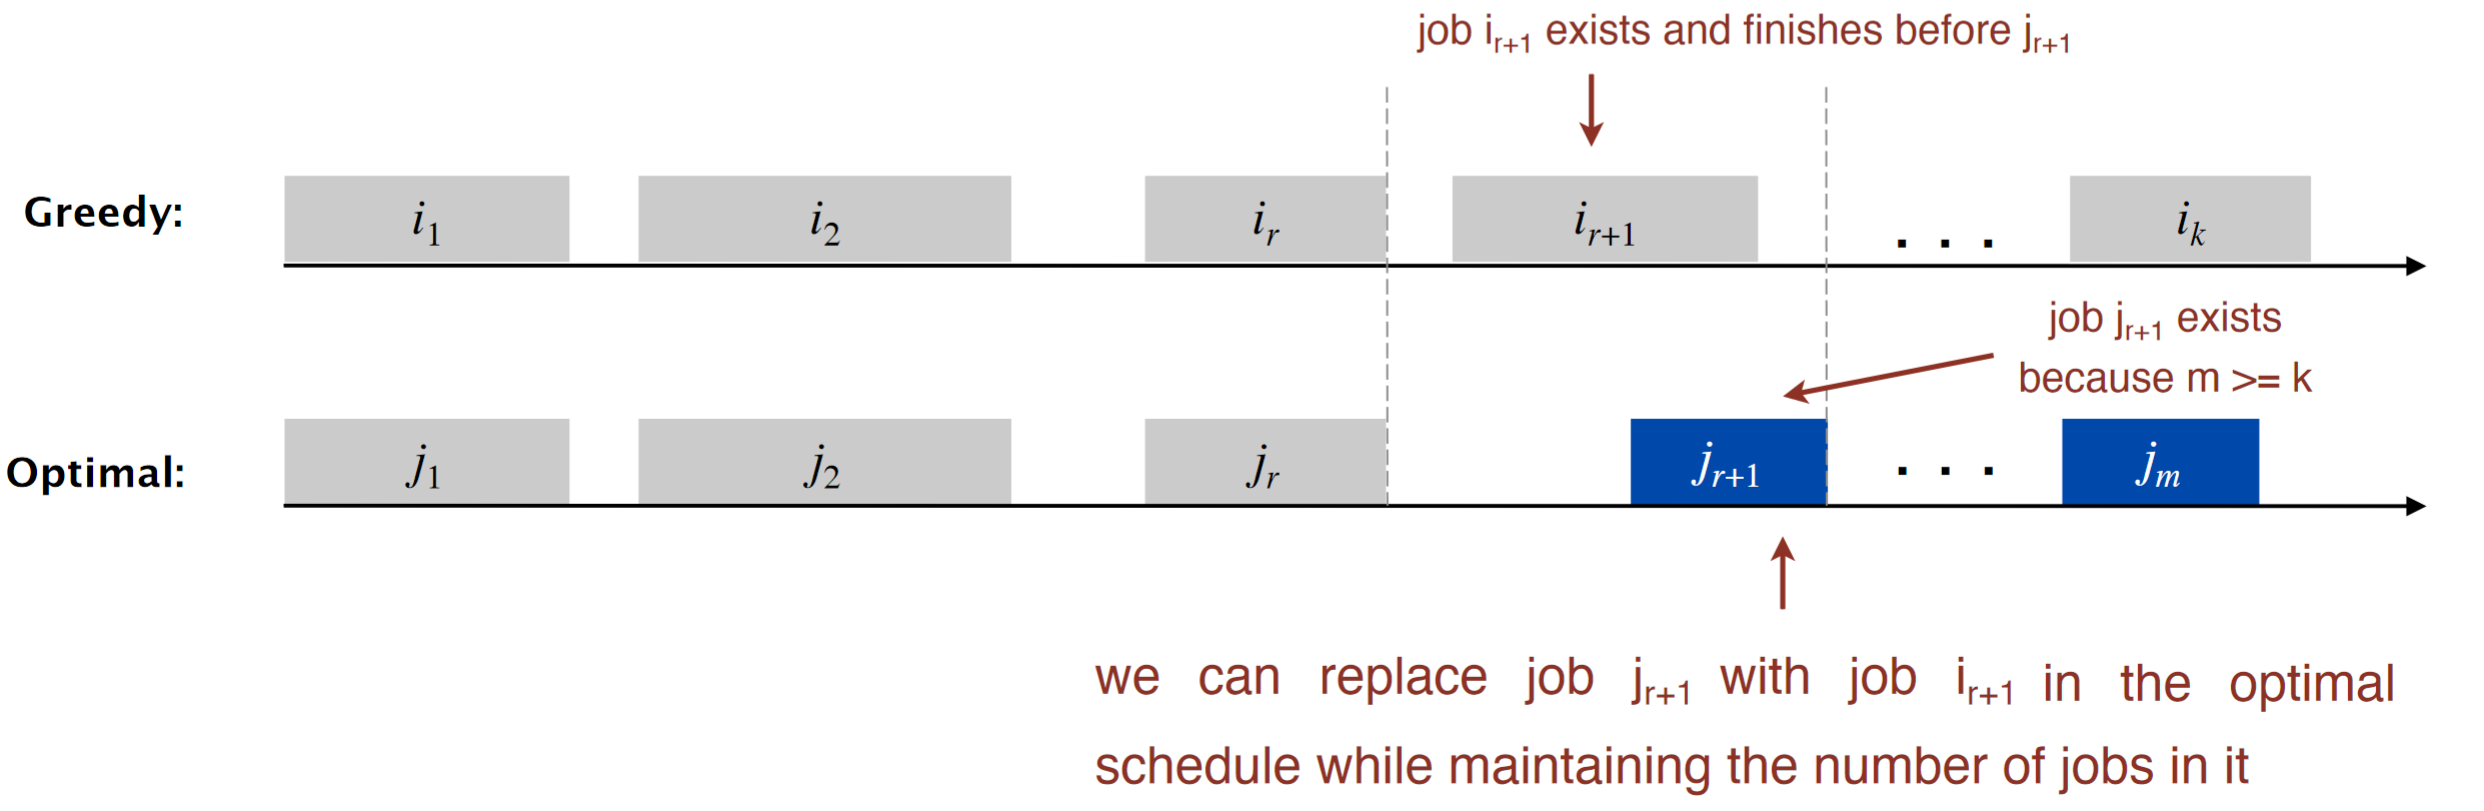
\includegraphics[height=1.7in]{./Sections/sched/interval/interval_proof.png}
    \end{center}
     \caption{Shows that at the first divergence, $i_{r+1}$ and .}\label{fig:interval_proof}
\end{figure}

\newpage 

\noindent
\begin{theo}[Interval Scheduling \& Earliest Finish Time]
    
    \label{thm:eft}
    Given a set of jobs $j$ with start and finish times $s_j$ and $f_j$, we can obtain an optimal like solution by scheduling in ascending order of $f_j$,
    choosing the next compatible job.
\end{theo}
\begin{figure}[h]
    \begin{center}
      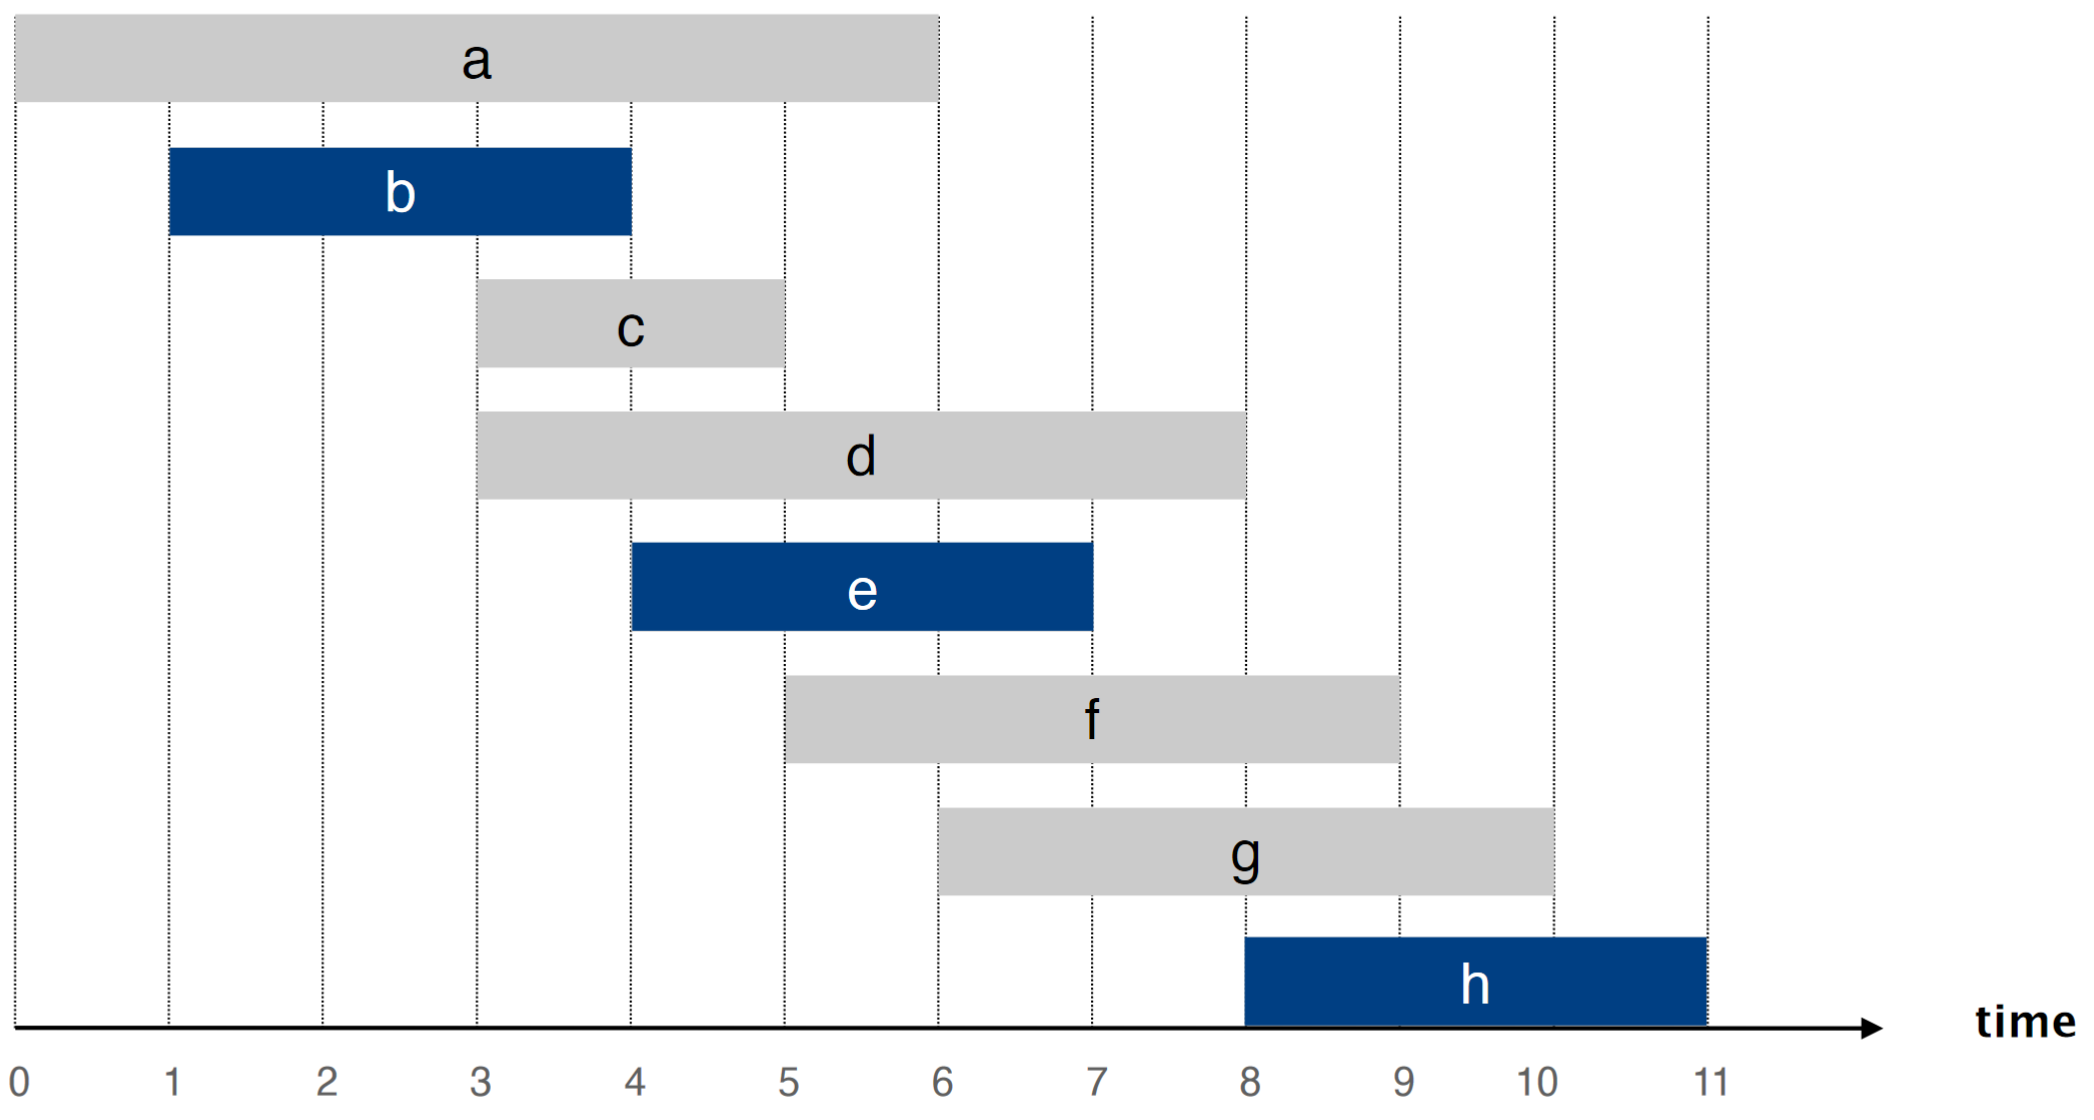
\includegraphics[height=2.3in]{./Sections/sched/interval/interval_sol.png}
    \end{center}
     \caption{Solution to Figure (\ref{fig:interval}) using early finish time first, yielding $\{b,e,h\}$.}\label{fig:interval_sol}
\end{figure}

\begin{Func}[EarliestFinishTimeFirst Algorithm - \texttt{EFT($s_1, \dots, s_n, f_1, \dots, f_n$)}]
    Finds the maximum set of non-overlapping jobs based on earliest finish time.

    \vspace{.5em}
    \noindent
    \textbf{Input:} A set of jobs with start times $s_j$ and finish times $f_j$.\\
    \textbf{Output:} The maximum set of selected jobs.\\
    \begin{algorithm}[H]
        \SetAlgoLined
        sorted\_jobs $\gets$ sort($f_1, \dots, f_n$) \tcp*[f]{sort by finish time}
        $S \gets \emptyset$ \tcp*[f]{selected jobs}
        $f_{\text{last}} \gets -\infty$\;

        \For{each $j$ in sorted\_jobs}{
            \If{$f_{\text{last}} \leq s_j$}{
                $S \gets S \cup \{j\}$\;
                $f_{\text{last}} \gets f_j$\;
            }
        }
        \KwRet{$S$}
    \end{algorithm}

    \noindent
    \textbf{Time Complexity:} $O(n\log n)$ assuming our sorting algorithm is $O(n\log n)$. Then we iterate through $n$ jobs.\\
    \textbf{Space Complexity:} $O(n)$ storing the input of $n$ jobs.
\end{Func}

\newpage
\section{Interval Partitioning}
Interval partitioning generalizes our interval scheduling to multiple resources, allowing them to run in parallel.

\begin{Def}[Interval Partitioning]
    
    Given a schedule of jobs $j$ with start and finish times $s_j$ and $f_j$. We \textbf{partition}
    jobs into a minimal amount of $k$ resources such that no two jobs on the same resource overlap.
\end{Def}
\textbf{Scenario: \textit{Class Scheduling}}\\
\noindent
Say we have $n$ classes and $k$ classrooms. What are the minimum number of classrooms needed to schedule all classes?\\


\noindent
\textbf{Example:} Let $n=\{a,b,c,\dots,i\}$ be classes with start and finish times. We attempt to find the minimum number of $k$ classrooms needed to schedule all classes.\\

\noindent
(1.)\label{ex:class_1}
\begin{figure}[h]
    \begin{center}
      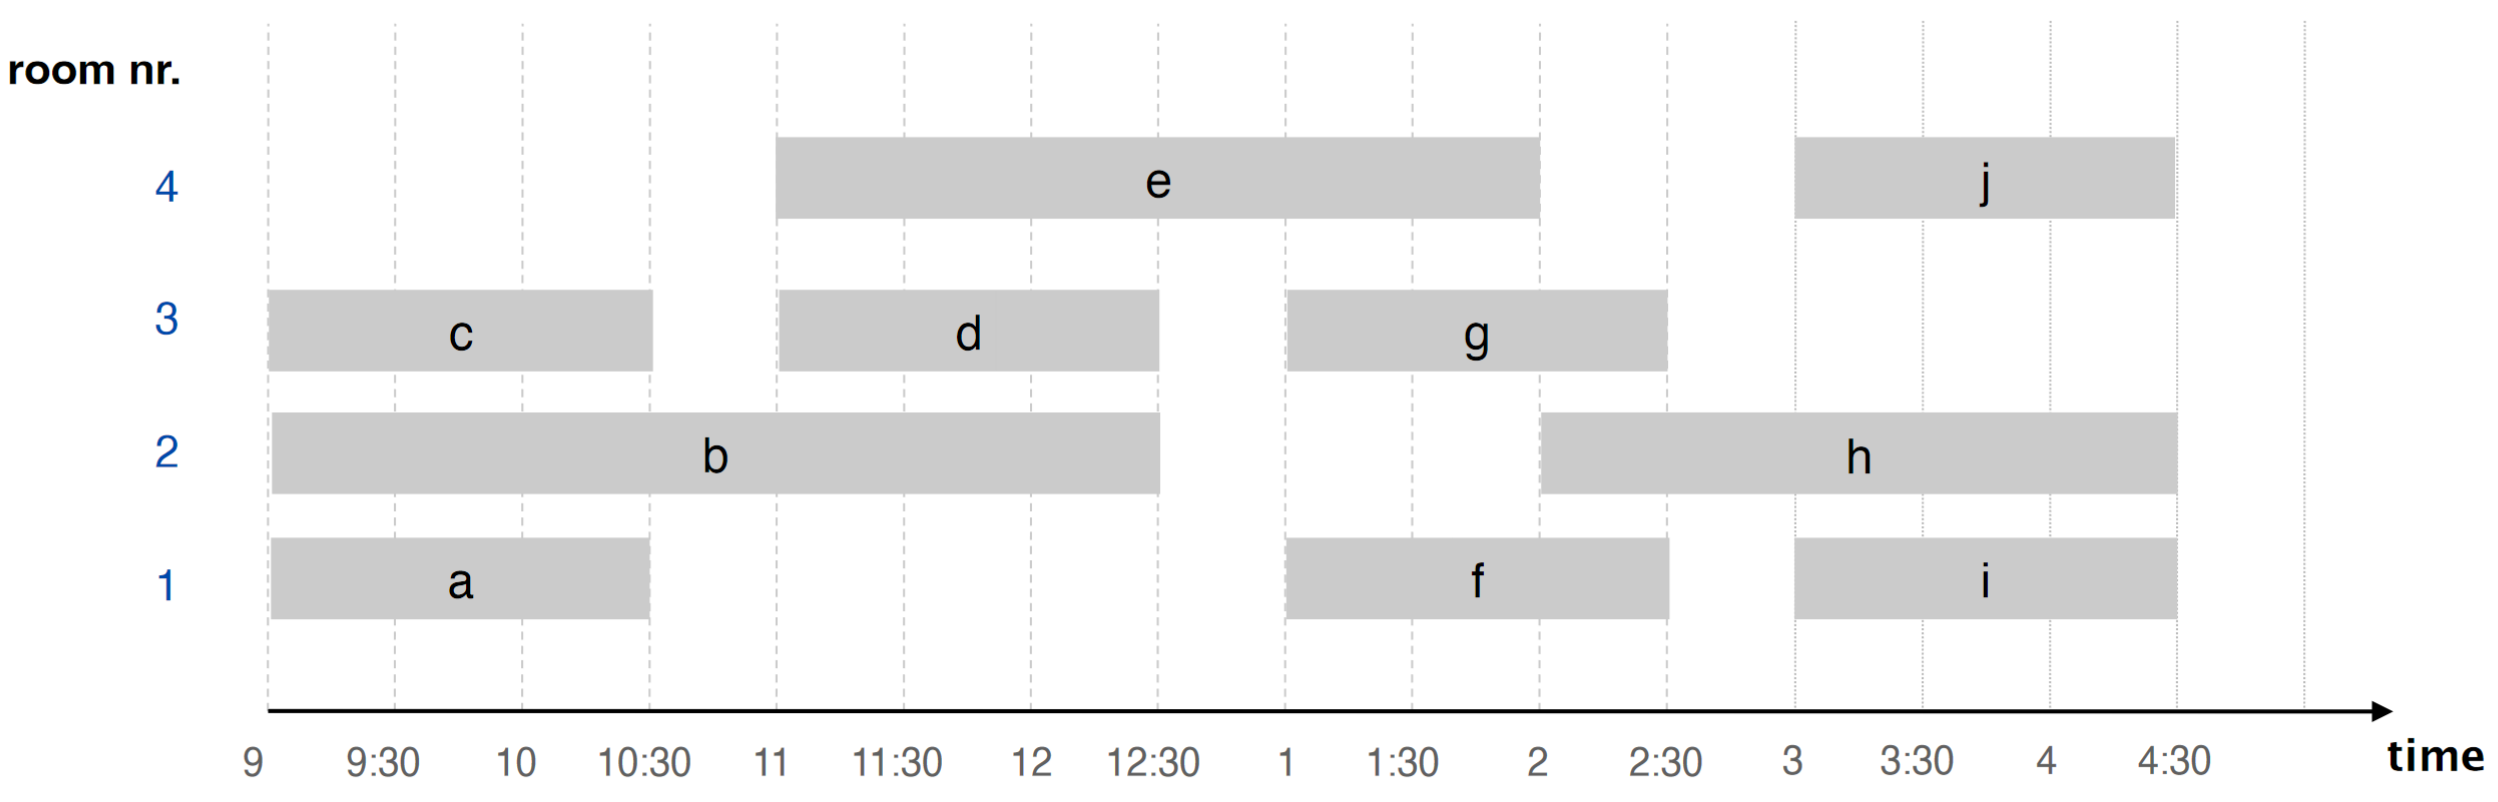
\includegraphics[height=2in]{./Sections/sched/interval/part/class_4.png}
    \end{center}
     \caption{Though not optimal, here is a possible schedule where $k=4$.}\label{fig:class_4}
\end{figure}

\noindent
We strategies and figure out the minimum number of classrooms needed to schedule all classes in the worst-case.
We observe in Example (\ref{ex:class_1}) that $\{c,b,a\}$ strictly overlap. Moreover, there are at most $3$ classes overlapping at any time. Thus, we need at least $3$ classrooms.\\
\begin{theo}[Minimality of Interval Partitioning]
    
    Given a set of jobs $j$, $c$ conflicting tasks, and $k$ resources. We find the 
    optimal $k$ by $k = \max(c)$.
\end{theo}

\newpage
\textbf{Possible Approaches:} Let $s_j$ and $f_j$ be the start and finish times of job $j$.
\begin{itemize}
    \item \textbf{[Earliest Start Time]:} Consider jobs in ascending order of $s_j$.
    \item \textbf{[Earliest Finish Time]:} Consider jobs in ascending order of $f_j$.
    \item \textbf{[Shortest Interval]:} Consider jobs in ascending order of $f_j - s_j$.
    \item \textbf{[Fewest Conflicts]:} For each $j$, count the number of conflicting jobs $c_j$. Schedule in ascending order of $c_j$.
\end{itemize}
\begin{theo}[Interval Partitioning \& Earliest Start Time]

    \label{theo:est}

    Given a set of jobs $j$ with start and finish times $s_j$ and $f_j$, we can obtain an optimal like solution by scheduling in ascending order of $s_j$.
    If two jobs overlap, we allocate a new resource.
\end{theo}

\vspace{-.5em}
\begin{figure}[h]
    \begin{center}
      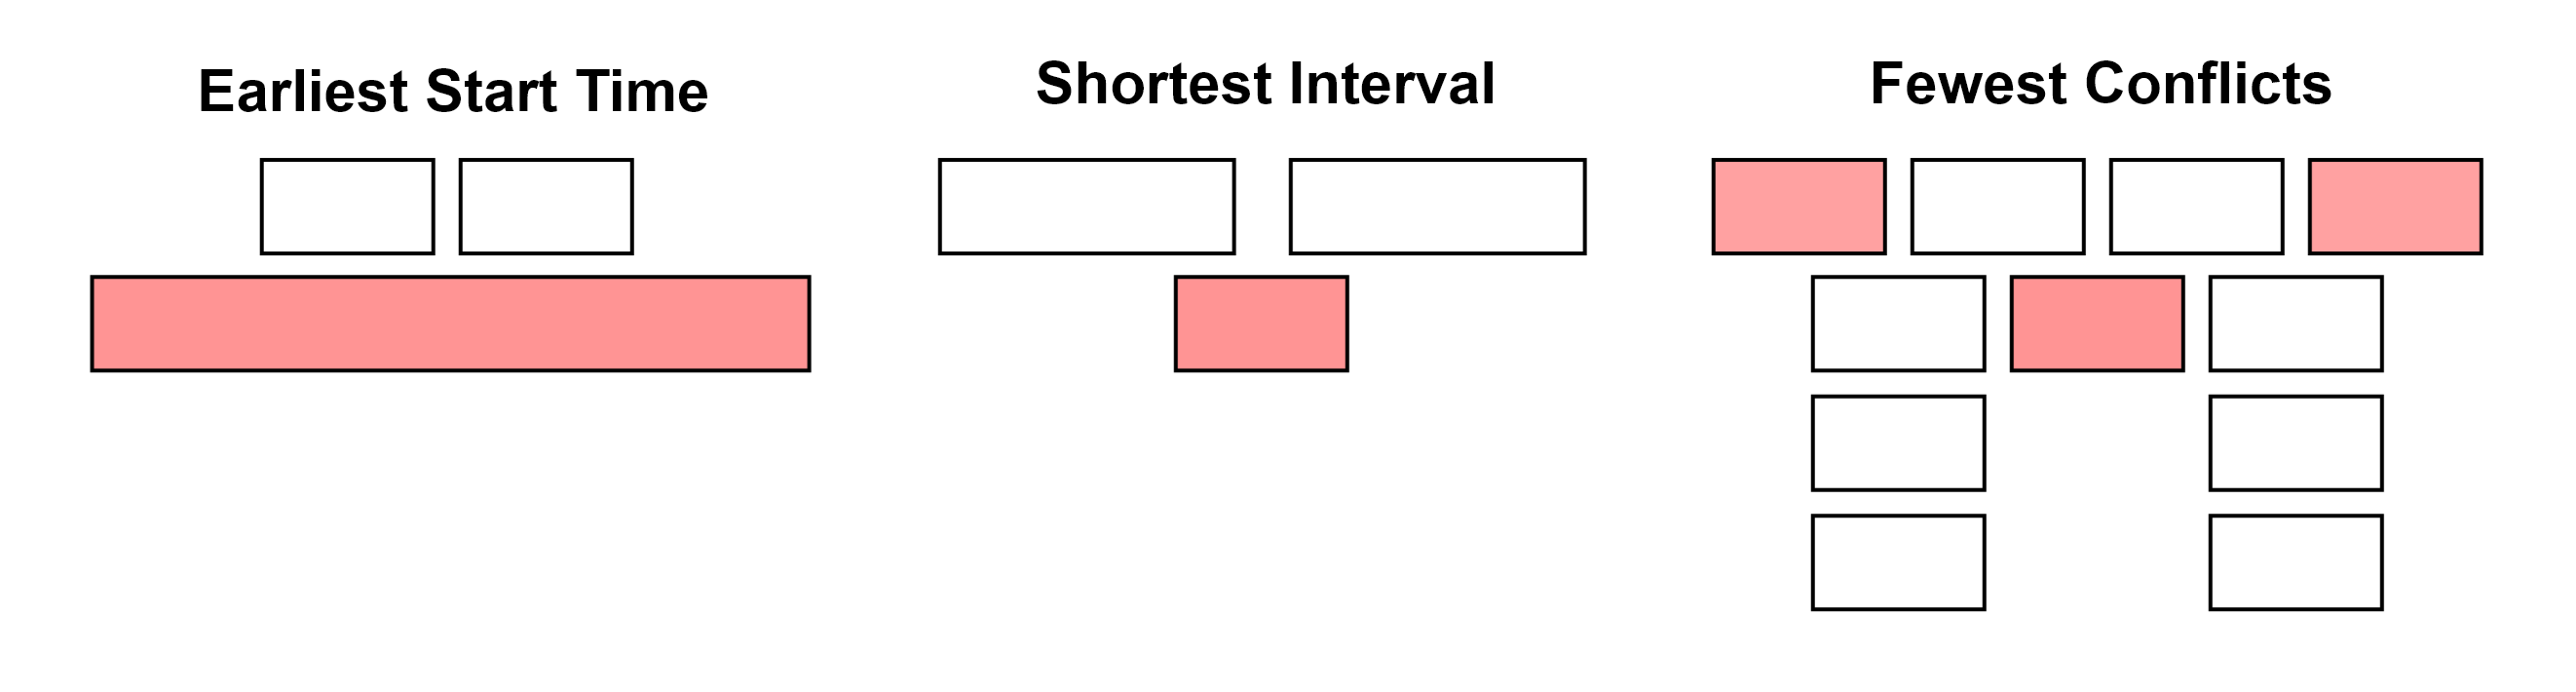
\includegraphics[width=\textwidth]{./Sections/sched/interval/counter.png}
    \end{center}
     
    \vspace{-.5em}
    \caption{Counter examples of Earliest Start Time, Shortest Interval, and Fewest Conflicts.
     Earliest time fails to see the later two smaller jobs, shortest interval fails to see two longer jobs, fewest 
     conflicts fails to see the sequential solution of 4 jobs because it has too many conflicts.}\label{fig:counter}
\end{figure}

\begin{Proof}[Classroom Allocation by Early Start Time First]
    Let $d$ be the number of classrooms that the algorithm allocates:

    \begin{enumerate}
        \item [(i.)] Classroom $d$ is opened because we needed to schedule a lecture, say $j$, that is incompatible with all $d - 1$ other classrooms.
        \item [(ii.)] These $d$ lectures each end after $s_j$.
        \item [(iii.)] Since we sorted by start time, all these incompatibilities are caused by lectures that start no later than $s_j$.
    \end{enumerate}
    \noindent
    All schedules use $\geq d$ classrooms. Thus, we have $d$ lectures overlapping at time $s_j + \epsilon$.

    \end{Proof}


    \newpage
    \begin{Func}[EarliestStartTimeFirst Algorithm - \texttt{EST($j = 1 \dots n : s_j, f_j$)}]
        Finds an optimal schedule of lectures based on their earliest start time.
        
        \vspace{.5em}
        \noindent
        \textbf{Input:} A set of lectures with start times $s_j$ and finish times $f_j$.\\
        \textbf{Output:} Assignment of lectures to rooms.\\
        \begin{algorithm}[H]
            \SetAlgoLined
            $\mathcal{A} \gets$ empty hash table \tcp*[f]{$\mathcal{A}[k]$ contains the list of lectures assigned to room $k$}
            sorted\_class $\gets$ sort($s_1, \dots, s_n$) \tcp*[f]{sort lectures by start time}
            
            \For{each $c$ in sorted\_class}{
                $k \gets$ find\_compatible\_room($c$, $\mathcal{A}$, $Q$)\;
                \If{$k$ is not None}{
                    $\mathcal{A}[k]$.add($c$)\;
                }
                \Else{
                    $d \gets$ len($\mathcal{A}$) \tcp*[f]{highest room id}
                    $\mathcal{A}[d + 1] \gets [\ ]$ \tcp*[f]{open new room}
                    $\mathcal{A}[d + 1]$.add($c$)\;
                }
            }
            \KwRet{$\mathcal{A}$}
        \end{algorithm}

        \noindent
        \textbf{Time Complexity:} $O(n\log n)$ assuming our sorting algorithm is $O(n\log n)$. Then we iterate through $n$ jobs.\\
        \textbf{Space Complexity:} $O(n)$ storing the input of $n$ jobs.
    \end{Func}

    
    
    
